\section{Les groupes}\label{sec:cree-un-groupe-d-utilisateurs-et-de-capteurs}

    \subsection{Fontionnement des groupes}\label{subsec:fontionnement-des-groupes}

        Pour permettre l'accès aux capteurs et leurs modifications des groupes ont été implémenter dans le logiciel.
        Il fonctionne de la manière suivante :
        Vous pouvez créé un groupe social permettant d'ajouter des membres et des capteurs en lecture seule.
        Dans ce groupe vous pouvez nommer un responsable et ainsi lui permettre de gérer le groupe.
        Vous pouvez créé un groupe de maintenance permettant d'ajouter capteurs et des membres qui pourront modifier ces capteurs
        et accéder à des informations permettant la mise en place et la maintenance des capteurs.
        Dans ce groupe vous pourrez nommer un responsable qui pourra ajouter ou supprimer des membres ainsi que des capteurs.
        Attention, ajouter un responsable lui permettra d'ajouter tous les capteurs du groupe à un groupe qu'il créera lui-même
        et sur lequel vous n'aurez aucun pouvoir.

        \begin{figure}[H]
            \begin{center}
                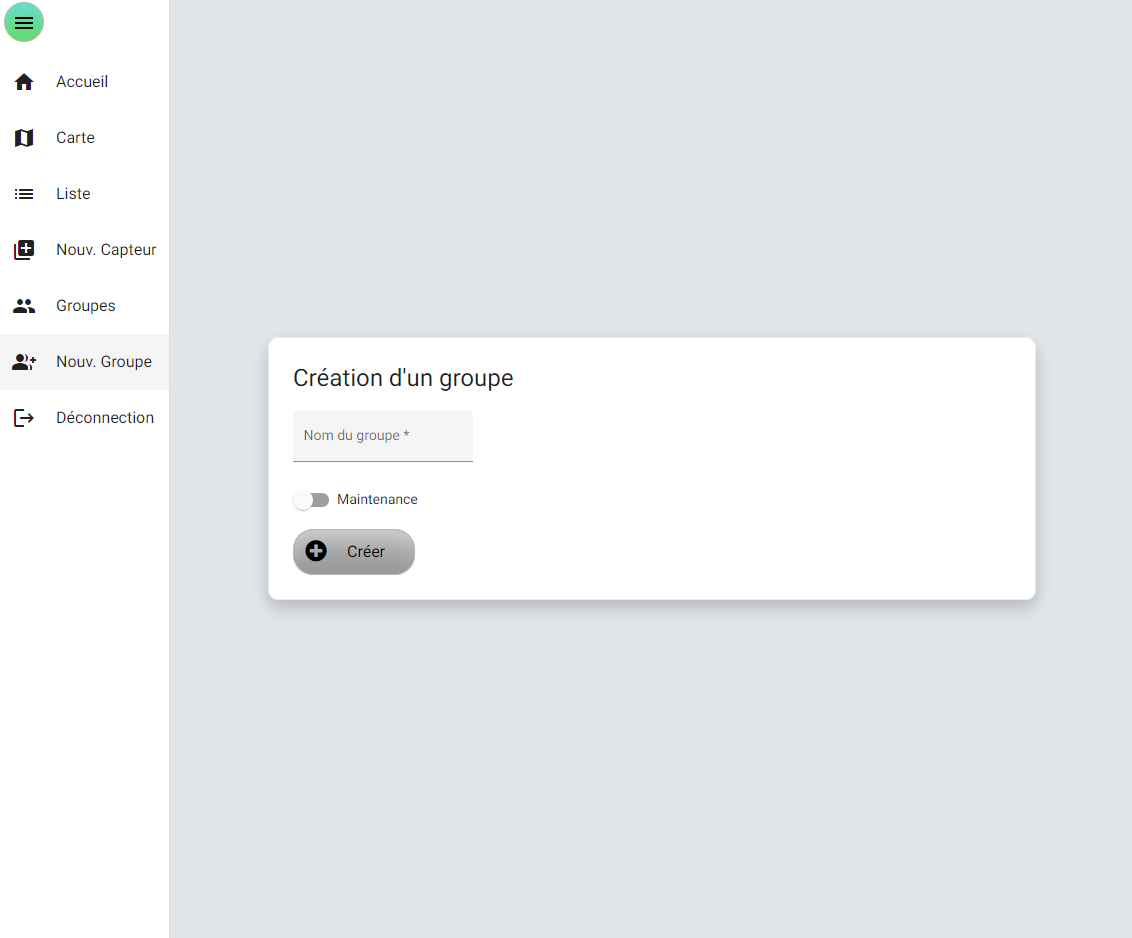
\includegraphics[width=12cm]{resources/create_group}
            \end{center}
            \caption{Page de création de groupe}\label{fig:create-group}
        \end{figure}

    \subsection{Créer un groupe}\label{subsec:creer-un-groupe}

        Pour créer un groupe vous devez être connecté, puis aller dans ``Nouv. Groupe''.
        Une fois ceci fait, vous devrez remplir le nom puis choisir si le groupe est de maintenance ou non.
        Pour terminer appuyer sur créer.

    \subsection{Rechercher un groupe}\label{subsec:rechercher-un-groupe}

        \begin{figure}[H]
            \begin{center}
                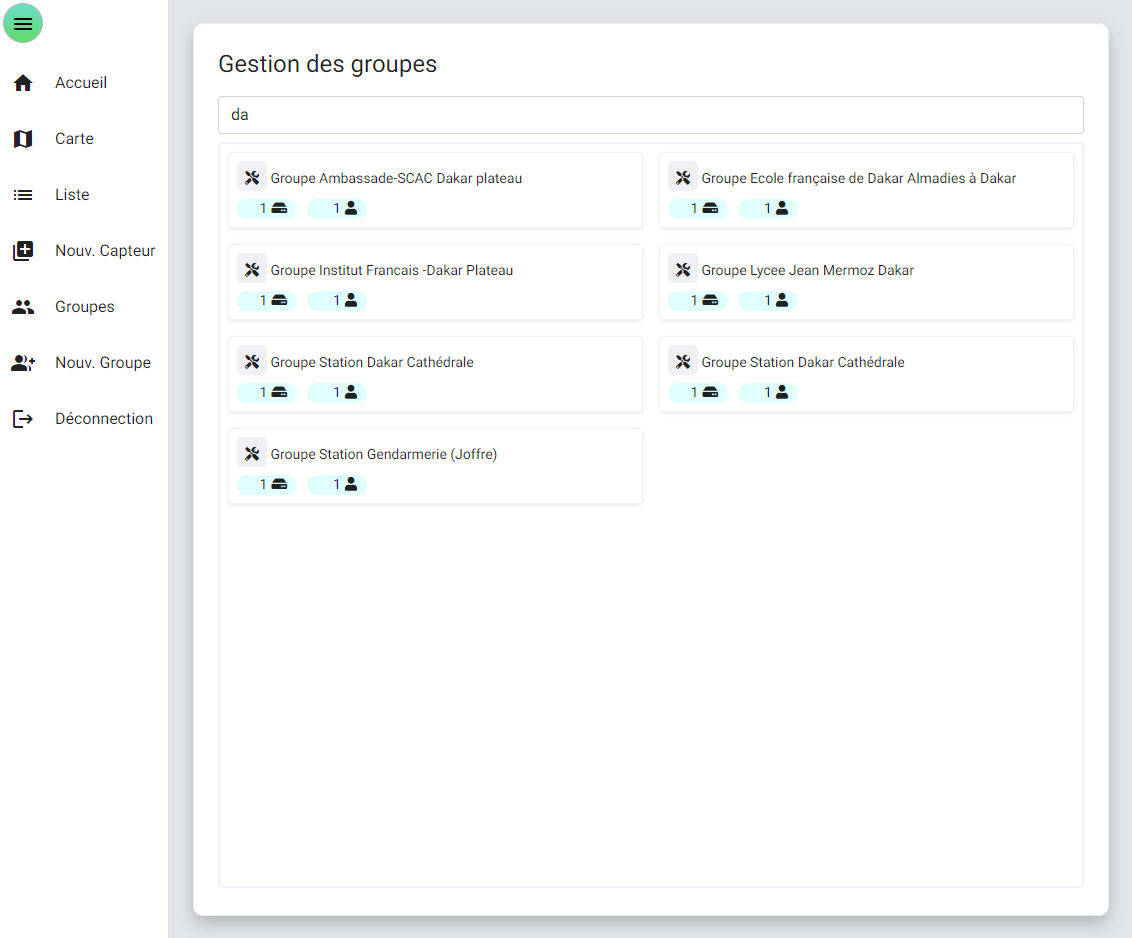
\includegraphics[width=12cm]{resources/group_search}
            \end{center}
            \caption{Rechercher un groupe}\label{fig:group-search}
        \end{figure}

        Afin de rechercher un groupe vous devez dans un premier temps être connecté et vous rendre dans l'onglet ``Groupes''.
        Vous pouvez sélectionner un groupe directement ou entrer le nom du groupe voulu dans la barre de recherche où il est indiqué ``Rechercher''.
        Une fois que vous avez clicker dessus vous retrouverez sur la page de gestion du groupe ci-dessous.


    \subsection{Gérer un groupe}\label{subsec:gerer-un-groupe}

        \begin{figure}[H]
            \begin{center}
                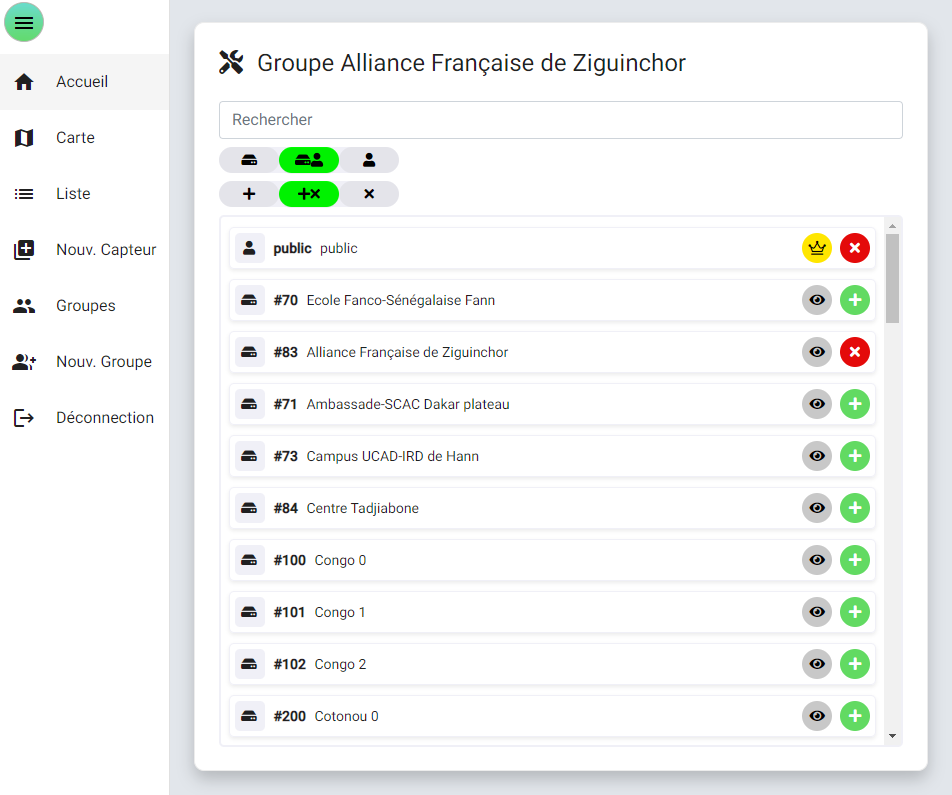
\includegraphics[width=12cm]{resources/group_manage}
            \end{center}
            \caption{Gérer un groupe}\label{fig:group-manage}
        \end{figure}

        Une fois sur cette page, vous pouvez choisir d'afficher seulement les utilisateurs, les capteurs ou les deux.
        Mais aussi choisir d'afficher les entitées (Capteur / membre) présentes dans le groupes, absent du groupe ou les deux.
        Ensuite pour chaque utilisateur vous pourrez choisir de l'ajouter au groupe ainsi que le supprimer ou le promouvoir s'il et déjà présent.
        Pour les capteurs ous pouvez accéder à leurs pages et les ajouter /supprimer du groupe.
